\documentclass[12pt]{../UWMadThesis}


% =============================================================================================== %
%                                     Math Commands                                               %
% =============================================================================================== %


% ---------------------------------------------------------------------------- %
%                                Square Root Tail                              %
% ---------------------------------------------------------------------------- %
\DeclareRobustCommand{\NthRootInTeX}[2]{\root #1 \of {#2\:\!}}

\DeclareRobustCommand{\SquareRootCore}[2]{
    \setbox0=\hbox{\ensuremath{\NthRootInTeX{#1}{#2}}}
    \dimen0=\ht0
    \advance\dimen0-0.2\ht0
    \setbox2=\hbox{\vrule height\ht0 depth -\dimen0}
    {\box0\lower0.47pt\box2}
}

\DeclareRobustCommand{\Sqrt}[2][]{
    \mathchoice{\SquareRootCore{#1}{#2}}
               {\SquareRootCore{#1}{#2}}
               {\SquareRootCore{#1}{#2}}
               {\SquareRootCore{#1}{#2}}
}



% ---------------------------------------------------------------------------- %
%                              Derivative Commands                             %
% ---------------------------------------------------------------------------- %
\newcommand{\bigdiffn}[4]{\dfrac{#1{}^{#4}}{#1 #3{}^{#4}} \left[ #2 \right]}
\newcommand{\gendiffn}[4]{\dfrac{#1{}^{#4} #2}{#1 #3{}^{#4}}}

\newcommand{\diff}[3][d]{
    \ifthenelse{\equal{p}{#1}}{
        \gendiffn{\partial}{#2}{#3}{}
    }{
        \ifthenelse{\equal{b}{#1}}{
            \bigdiffn{d}{#2}{#3}{}
        }{
            \ifthenelse{\equal{bp}{#1}}{
                \bigdiffn{\partial}{#2}{#3}{}
            }{
                \gendiffn{d}{#2}{#3}{}
            }
        }
    }
}

\newcommand{\diffn}[4][d]{
    \ifthenelse{\equal{p}{#1}}{
        \gendiffn{\partial}{#2}{#3}{#4}
    }{
        \ifthenelse{\equal{b}{#1}}{
            \bigdiffn{#2}{#3}{#4}
        }{
            \ifthenelse{\equal{bp}{#1}}{
                \bigdiffn{\partial}{#2}{#3}{#4}
            }{
                \gendiffn{#1}{#2}{#3}{#4}
            }
        }
    }
}

\newcommand{\bigdiff}   [2] {\diff[b]{#1}{#2}}
\newcommand{\pdiff}     [2] {\diff[p]{#1}{#2}}
\newcommand{\bigpdiff}  [2] {\diff[bp]{#1}{#2}}
\let\frac\dfrac
\newcommand{\subs}      [2][]{\ensuremath{{}_{#1\text{\scriptsize #2}}}}
\newcommand{\sups}      [2][]{\ensuremath{{}^{#1\text{\scriptsize #2}}}}
\newcommand{\oneo}      [1]  {\ensuremath{\frac{1}{#1}}}




\newcommand{\Density}{\ensuremath{\rho}\xspace}
\newcommand{\Temperature}{\ensuremath{T}\xspace}
\newcommand{\Pressure}{\ensuremath{P}\xspace}
\newcommand{\IntEnergy}{\ensuremath{i}\xspace}
\newcommand{\Entropy}{\ensuremath{s}\xspace}
\newcommand{\Enthalpy}{\ensuremath{h}\xspace}
\newcommand{\ThCond}{\kappa}
\newcommand{\Viscosity}{\mu}
\newcommand{\DiffCoef}{\ensuremath{D}\xspace}

\newcommand{\isat}{\ensuremath{\IntEnergy\subs[\!]{sat}}\xspace}
\newcommand{\Psat}{\ensuremath{\Pressure\subs[\!\!]{sat}}\xspace}
\newcommand{\Tsat}{\ensuremath{\Temperature\subs[\!\!\:]{sat}}\xspace}
\newcommand{\SubL}{\subs[\!\!\:]{\rule{0pt}{8pt}$\textstyle\ell$}}
\newcommand{\SubG}{\subs[\!\!\:]{$\mathit{g}$}}

\newcommand{\rhol}{\ensuremath{\rho\SubL}\xspace}
\newcommand{\rhog}{\ensuremath{\rho\SubG}\xspace}
\newcommand{\il}{\ensuremath{i\SubL}\xspace}
\newcommand{\ig}{\ensuremath{i\SubG}\xspace}
\newcommand{\rhoul}{\ensuremath{\rhou\SubL}\xspace}
\newcommand{\rhoug}{\ensuremath{\rhou\SubG}\xspace}
\newcommand{\rhoil}{\ensuremath{\rhoi\SubL}\xspace}
\newcommand{\rhoig}{\ensuremath{\rhoi\SubG}\xspace}
\newcommand{\alphal}{\ensuremath{\alpha\SubL}\xspace}
\newcommand{\alphag}{\ensuremath{\alpha\SubG}\xspace}

\newcommand{\tauSat}{\ensuremath{\tau\subs[\!\!\:]{sat}}\xspace}
\newcommand{\deltaL}{\ensuremath{\delta\subs[\!\!\:]{\rule{0pt}{8pt}$\textstyle\ell$}}\xspace}
\newcommand{\deltaG}{\ensuremath{\delta\subs[\!\!\:]{$\mathit{g}$}}\xspace}

\newcommand{\rhoc}  {\ensuremath{\rho\subs{c}}\xspace}
\newcommand{\Tc}    {\ensuremath{T\subs{c}}\xspace}

\newcommand{\Skip}[1][0.45em]{\\[#1]}
\newcommand{\TCS}    {Thermodynamic Coexistence System\xspace}
\newcommand{\TCSRef} {\hyperref[Eqn:TCS]{\TCS}\xspace}
\newcommand{\MCS}    {Mechanical Coexistence System\xspace}
\newcommand{\MCSRef} {\hyperref[Eqn:MCS]{\MCS}\xspace}

\newcommand{\Afe}{\ensuremath{A\subs{\textsc{fe}}}}
\newcommand{\HFE}{Helmholtz free energy\xspace}
\newcommand{\EOS}{equation of state\xspace}

\newcommand{\Space}{\ensuremath{z}\xspace}
\newcommand{\Time}{\ensuremath{t}\xspace}
\newcommand{\Speeds}{\ensuremath{\mathbf{\lambda}}\xspace}

\DeclareMathOperator{\Ln}{Ln}
\DeclareMathOperator{\Abs}{Abs}
\DeclareMathOperator{\Inf}{Inf}
\DeclareMathOperator{\Exp}{Exp}
\DeclareMathOperator{\Rez}{R}

\let\originalleft\left
\let\originalright\right
\renewcommand{\left}{\mathopen{}\mathclose\bgroup\originalleft\;\!}
\def\left#1{\mathopen{}\mathclose\bgroup\originalleft#1\:\!}
\def\right#1{\aftergroup\egroup\:\!\originalright#1}


%\DefineNewLength{\RowSkip}{1.0em}
%\newcommand{\skp}[1][0.45em]{
%    \ifthenelse{\equal{#1}{}}{
%        \\[\RowSkip]
%    }{
%        \\[#1]
%    }
%}

\newcommand{\Del}[1][]{
    \partial_{#1}
}

\newcommand{\Vector}[1]{
    \underline{#1}
}

\newcommand{\Tensor}[1]{
    \underline{\underline{#1}}
}

\newcommand{\qConRaw}{\mathbf{q}}
\newcommand{\qCon}{\ensuremath{\qConRaw}\xspace}
\newcommand{\qPer}{\ensuremath{\widehat{\qConRaw}}\xspace}
\newcommand{\qSS} {\ensuremath{\qConRaw^0}\xspace}

\newcommand{\ConSys}{
    \Psi
}

\newcommand{\ConSysHEM}[1][HEM]{
    \ConSys_{\!\mbox{\tiny #1}}
}


\newcommand{\Flux}{
    \mathbf{F}
}
\newcommand{\Source}{
    \mathbf{S}
}

\newcommand{\Weight}{\beta}


\newcommand{\FluxFun}[2][]{
    \mathbf{F}_{#1}\left(#2\right)
}

\newcommand{\SourceFun}[2][]{
    \mathbf{S}_{#1}\left(#2\right)
}

\newcommand{\ResidualFun}[2][]{
    \mathbf{R}_{#1}\left(#2\right)
}

\newcommand{\Jacobian}[1][]{
    \mathbb{J}\subs{#1}
}

\newcommand{\JacobGen}[2]{
  \Jacobian[{\scriptscriptstyle #1}](#2)
}

\newcommand{\JacobF}{
    \Jacobian[F]
}


\newcommand{\JacobS}[1]{
    \JacobGen{S}{#1}
}

\newcommand{\FluxSS}{
    \mathbf{F}^{0}
}

\newcommand{\SourceSS}{
    \mathbf{S}^{0}
}

\newcommand{\JacobFSS}[1][\,\,\!]{
    \mathbf{J}_{\!{\scriptscriptstyle F}}^{0}{}#1
}

\newcommand{\JacobSSS}[1][\,\,\!]{
    \mathbf{J}_{\!{\scriptscriptstyle S}}^{0}#1
}

\newcommand{\BigO}[1]{
    \ensuremath{\mathcal{O}\!\left(#1\right)}
}


\newcommand{\Correl}[2]{
    f^{\mbox{\scriptsize cor}}_{#1}\left(#2\right)
}

\newcommand{\LpNorm}[2][2]{
    \ensuremath{\lvert\!\lvert#2\rvert\!\rvert_{#1}}
}

\newcommand{\Nudge}{
    \ensuremath{\!\!\;}
}

\newcommand{\hfg}{
    \ensuremath{h_{\mbox{\scriptsize fg}}}
}



%\NewEnviron{BoxedAlgorithm}[1][H]{
%    \begin{center}
%        \begin{minipage}{0.999\textwidth}
%            \centering
%            \fcolorbox{black}{white}{
%                \centering
%                \begin{minipage}[t]{0.85\textwidth}
%                    \begin{algorithm}[#1]
%                        \BODY
%                    \end{algorithm}
%                \end{minipage}
%            }
%        \end{minipage}
%    \end{center}
%}


\DeclareRobustCommand{\TH}  {thermal hydraulics\xspace}
\DeclareRobustCommand{\THc} {Thermal hydraulics\xspace}
\DeclareRobustCommand{\THcc}{Thermal Hydraulics\xspace}
\DeclareRobustCommand{\THs} {thermal hydraulic\xspace}

\DeclareRobustCommand{\CLaw}  {conservation law\xspace}
\DeclareRobustCommand{\CLaws} {conservation laws\xspace}


\newcommand{\rhou}{\ensuremath{\rho{u}}\xspace}
\newcommand{\rhoi}{\ensuremath{\rho{i}}\xspace}

\newcommand{\tr}{\ensuremath{{}\sups{\textsc{T}}}}
\newcommand{\mdotloss}[1][]{\ensuremath{\dot{m}'''\subs[\!\!\!\!\!#1]{loss}}\xspace}
\newcommand{\Keff}{\ensuremath{K\subs{eff}}}

\newcommand{\POfRhoRhoi}{\ensuremath{P\left(\rho,\frac{\rhoi}{\rho}\right)}}


\newcommand{\EqnSkip}[1][3em]{\ensuremath{\mbox{\rule{0.5em}{#1}}}\\}
\newcommand{\psiEOS}{\ensuremath{\psi}\subs{\textsc{eos}}}




%\DefineNewLength{\BarredLetterHeight}{0pt}
%\DefineNewLength{\BarredLetterWidth}{0pt}

%\newcommand{\eBB}{
%    \ensuremath{
%        \settoheight{\BarredLetterHeight}{e} % Height in current context
%        \settowidth{\BarredLetterWidth}{e}   % Width  in current context
%        e\mbox{\hspace{-0.57\BarredLetterWidth}\rule{0.035em}{0.96\BarredLetterHeight}} % bar
%    }
%}

%\newcommand{\TableSkip}{\rule[-1.4em]{0pt}{3.3em} \\[0pt]}
\definecolor{Gray}{gray}{0.93}


\newcommand{\LedineggCriterion}{$\tfrac{\partial\Delta{P}}{\partial(\rhou)}\bigr\rvert_{\text{int}} \le 
                                 \tfrac{\partial\Delta{P}}{\partial(\rhou)}\bigr\rvert_{\text{ext}}$}
                                
                                
\newcommand{\etal}{et al.\xspace}
\newcommand{\etc}{etc.\xspace}
\newcommand{\eg}{e.g.\xspace}
\newcommand{\ie}{i.e.\xspace}


\newcommand{\rhok}{ \ensuremath{\alpha\rho\subs{\phi}}\xspace}
\newcommand{\rhouk} {\ensuremath{\alpha\rhou\subs{\phi}}\xspace}
\newcommand{\rhoik} {\ensuremath{\alpha\rhoi\subs{\phi}}\xspace}
\newcommand{\alphak}{\ensuremath{\alpha\subs{\phi}\xspace}}
\newcommand{\uk}{\ensuremath{u\subs{\phi}}\xspace}
\newcommand{\ik}{\ensuremath{i\subs{\phi}}\xspace}
\newcommand{\CVvol}[1][k]{\ensuremath{\Omega_\text{#1}}\xspace}
\newcommand{\MCvol}[1][m]{\ensuremath{\Omega_\text{#1}}\xspace}
\newcommand{\CVsurf}[1][k]{\ensuremath{\Gamma_\text{#1}}\xspace}
\newcommand{\MCsurf}[1][m]{\ensuremath{\Gamma_\text{#1}}\xspace}








    \let\Oldalpha     \alpha     \renewcommand{\alpha}     {\ensuremath{\Oldalpha     }\xspace}
    \let\Oldbeta      \beta      \renewcommand{\beta}      {\ensuremath{\Oldbeta      }\xspace}
    \let\Oldgamma     \gamma     \renewcommand{\gamma}     {\ensuremath{\Oldgamma     }\xspace}
    \let\Olddelta     \delta     \renewcommand{\delta}     {\ensuremath{\Olddelta     }\xspace}
    \let\Oldepsilon   \epsilon   \renewcommand{\epsilon}   {\ensuremath{\Oldepsilon   }\xspace}
    \let\Oldvarepsilon\varepsilon\renewcommand{\varepsilon}{\ensuremath{\Oldvarepsilon}\xspace}
    \let\Oldzeta      \zeta      \renewcommand{\zeta}      {\ensuremath{\Oldzeta      }\xspace}
    \let\Oldeta       \eta       \renewcommand{\eta}       {\ensuremath{\Oldeta       }\xspace}
    \let\Oldtheta     \theta     \renewcommand{\theta}     {\ensuremath{\Oldtheta     }\xspace}
    \let\Oldvartheta  \vartheta  \renewcommand{\vartheta}  {\ensuremath{\Oldvartheta  }\xspace}
    \let\Oldkappa     \kappa     \renewcommand{\kappa}     {\ensuremath{\Oldkappa     }\xspace}
    \let\Oldlambda    \lambda    \renewcommand{\lambda}    {\ensuremath{\Oldlambda    }\xspace}
    \let\Oldmu        \mu        \renewcommand{\mu}        {\ensuremath{\Oldmu        }\xspace}
    \let\Oldnu        \nu        \renewcommand{\nu}        {\ensuremath{\Oldnu        }\xspace}
    \let\Oldxi        \xi        \renewcommand{\xi}        {\ensuremath{\Oldxi        }\xspace}
    \let\Oldpi        \pi        \renewcommand{\pi}        {\ensuremath{\Oldpi        }\xspace}
    \let\Oldvarpi     \varpi     \renewcommand{\varpi}     {\ensuremath{\Oldvarpi     }\xspace}
    \let\Oldrho       \rho       \renewcommand{\rho}       {\ensuremath{\Oldrho       }\xspace}
    \let\Oldvarrho    \varrho    \renewcommand{\varrho}    {\ensuremath{\Oldvarrho    }\xspace}
    \let\Oldsigma     \sigma     \renewcommand{\sigma}     {\ensuremath{\Oldsigma     }\xspace}
    \let\Oldvarsigma  \varsigma  \renewcommand{\varsigma}  {\ensuremath{\Oldvarsigma  }\xspace}
    \let\Oldtau       \tau       \renewcommand{\tau}       {\ensuremath{\Oldtau       }\xspace}
    \let\Oldupsilon   \upsilon   \renewcommand{\upsilon}   {\ensuremath{\Oldupsilon   }\xspace}
    \let\Oldphi       \phi       \renewcommand{\phi}       {\ensuremath{\Oldphi       }\xspace}
    \let\Oldvarphi    \varphi    \renewcommand{\varphi}    {\ensuremath{\Oldvarphi    }\xspace}
    \let\Oldchi       \chi       \renewcommand{\chi}       {\ensuremath{\Oldchi       }\xspace}
    \let\Oldpsi       \psi       \renewcommand{\psi}       {\ensuremath{\Oldpsi}\xspace}
    \let\Oldomega     \omega     \renewcommand{\omega}     {\ensuremath{\Oldomega     }\xspace}
    \let\OldGamma     \Gamma     \renewcommand{\Gamma}     {\ensuremath{\OldGamma     }\xspace}
    \let\OldLambda    \Lambda    \renewcommand{\Lambda}    {\ensuremath{\OldLambda    }\xspace}
    \let\OldSigma     \Sigma     \renewcommand{\Sigma}     {\ensuremath{\OldSigma     }\xspace}
    \let\OldPsi       \Psi       \renewcommand{\Psi}       {\ensuremath{\OldPsi       }\xspace}
    \let\OldDelta     \Delta     \renewcommand{\Delta}     {\ensuremath{\OldDelta     }\xspace}
    \let\OldXi        \Xi        \renewcommand{\Xi}        {\ensuremath{\OldXi        }\xspace}
    \let\OldUpsilon   \Upsilon   \renewcommand{\Upsilon}   {\ensuremath{\OldUpsilon   }\xspace}
    \let\OldOmega     \Omega     \renewcommand{\Omega}     {\ensuremath{\OldOmega     }\xspace}
    \let\OldTheta     \Theta     \renewcommand{\Theta}     {\ensuremath{\OldTheta     }\xspace}
    \let\OldPi        \Pi        \renewcommand{\Pi}        {\ensuremath{\OldPi        }\xspace}
    \let\OldPhi       \Phi       \renewcommand{\Phi}       {\ensuremath{\OldPhi       }\xspace}


\usepackage{enumitem}

%   Graphics path definition
\UWMadSetup{
    RelativeDirectory / {
        the-only-graphics-directory = Graphics
    }
}

%   Shim until merged back into the full document
\renewcommand{\Acronym}[1]{#1}

\ExplSyntaxOn

    \tl_set_eq:Nc \l_tmpa_tl {Gin@extensions}
    \clist_new:N \g__UWMad_RelativeDirectory_ImageExtensions_clist
    \clist_set:No
        \g__UWMad_RelativeDirectory_ImageExtensions_clist
        {\l_tmpa_tl}

    %\clist_show:N \g__UWMad_RelativeDirectory_ImageExtensions_clist
    \tl_new:N   \l__UWMad_File_Path_tl
    \tl_new:N   \l__UWMad_File_Name_tl
    \tl_new:N   \l__UWMad_File_Extension_tl
    
    \def\l_tmpa_tl{path/file.ext}
    
    \UWMad_File_PathFileName:nnnx
        \l__UWMad_File_Path_tl
        \l__UWMad_File_Name_tl
        \l__UWMad_File_Extension_tl
        {\l_tmpa_tl/\l_tmpa_tl}
        
    \tl_if_blank:VTF {\l__UWMad_File_Path_tl} {
        \msg_term:n {The~path~is~empty!}
    } {
        \msg_term:n {The~path~is~\l__UWMad_File_Path_tl}
    }
    \tl_show:N \l__UWMad_File_Name_tl
    \tl_show:N \l__UWMad_File_Extension_tl

\ExplSyntaxOff



\Institution{University of Wisconsin--Madison}


\begin{document}

\chapter{Introduction}

Stability of two-phase natural circulation systems is not a novel subject in and of itself.
However, this work aims to perform analysis on a novel geometry with unique characteristics using rigorous numerical methods.
Motivation for this effort is given through the examination of an experimental facility and preliminary data, both experimental and numerical.
Then, a literature overview of the field of stability analysis of fluid systems is presented with a broader perspective than that of this work.
Finally, the chapter concludes with the end goals of this investigation and an outline of the work.

\iffalse
 
\section{Reactor Cavity Cooling System}\label{Section:RCCS}
The primary motivation behind this stability work is the so-called \Acronym{RCCS}, which is a safety system for certain proposed Generation IV reactor designs.
A definition and discussion of this safety system for full-scale application is discussed first and followed by a description of an experimental test facility at the \TheUniversity.

\subsection{Full-Scale System}
The \Acronym{NGNP} is a thermal-spectrum, gas-cooled reactor designed to be able to produce electricity as well as process heat for industrial applications.
A novel feature of the \Acronym{NGNP} is the \Acronym{RCCS}.
The \Acronym{RCCS} is a natural circulation system of ducts designed as the \Acronym{NGNP}'s ultimate heat sink for decay heat under a number of accident scenarios.
There are two main designs under consideration which vary mostly in their working fluid: air-cooled and water-cooled.
This work will focus on the water-cooled \Acronym{RCCS} design, leaving air-cooled discussions left to the literature \cite{bechtelnationalinc._450_1993,generalatomics_gas_1996}.


\begin{figure}%
\centering
    \caption[ANL/UW-Madison water-cooled RCCS diagram]{   ANL/UW-Madison  water-cooled RCCS diagram.  
                Water flows from a tank, through the cold leg (blue), through the reactor cavity system, and through the hot leg (red) to some tank on the train at the same conditions (a closed circuit).}%
    \label{Figure:RCCSTotalSystem}%
    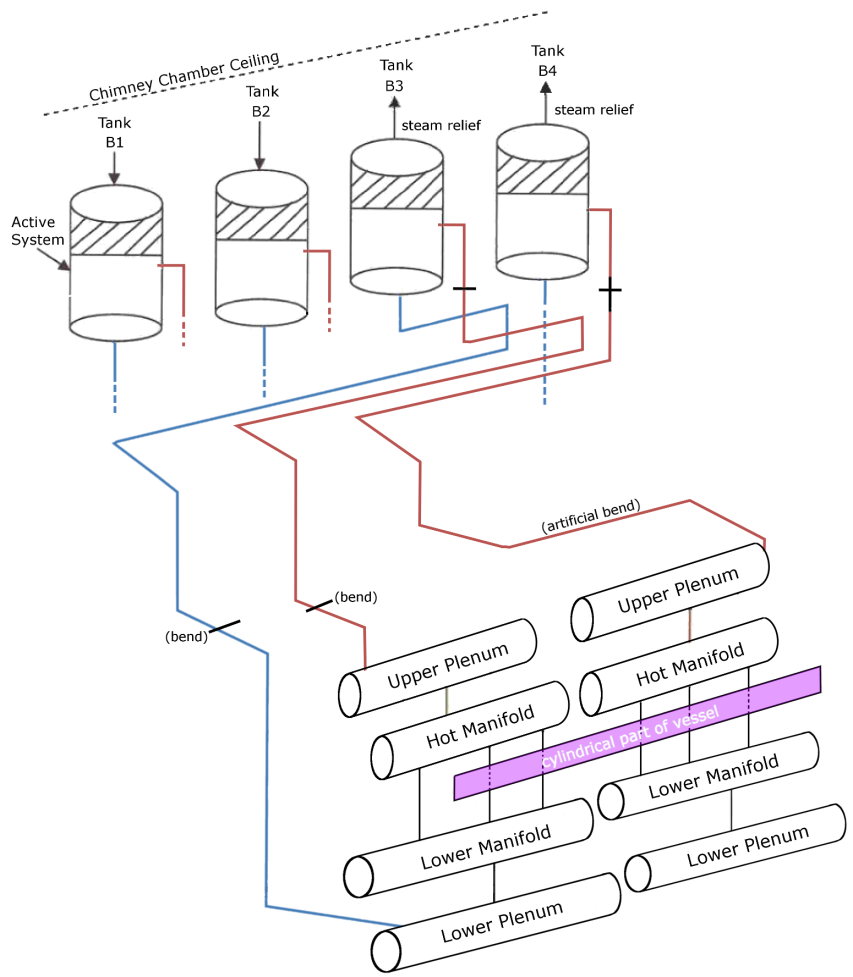
\includegraphics[scale=1.2]{RCCSTotalSystem.png}%
\end{figure}


A collaboration between \Acronym{ANL} and the \TheUniversity\ produced a base, full-scale \Acronym{RCCS} system consisting of a two independent piping networks with each network having four main lines/tanks.
\Cref{Figure:RCCSTotalSystem} outlines the basic design of system B but precludes any detail near the reactor.
The elevation change of the system is on the order of several tens of meters with the reactor cavity portion being approximately twenty meters on its own.
Within the reactor cavity, the eight cold lines of the \Acronym{RCCS} splits into approximately 200 so-called riser pipes that line the cavity wall and ensconce the reactor (see \cref{Figure:RCCSMockup}).
The riser pipes then receive heat from the uninsulated reactor pressure vessel via convection and radiation.
Due to the heating, the fluid that fills the pipes is subjected to a buoyancy force that results in upward flow.

During steady-state operation of the reactor, there is a persistent, parasitic heat loss from the reactor vessel to the \Acronym{RCCS} of approximately $700$ kW.
If the reactor undergoes a loss-of-forced-flow accident with SCRAM, there is an expected peak decay heat load of $1.5$ MW on the \Acronym{RCCS}.
If there is no loss of onsite or offsite power, the \Acronym{RCCS} water storage tanks will be actively cooled, and the system is expected to maintain safe fuel temperatures for the duration of the accident.
In the event of loss of onsite and offsite power (so-called station blackout), the \Acronym{RCCS} can still continue to cool the reactor since the flow is naturally circulating, which is very important for the overall safety of the plant \cite[\SS{50.63}]{nuclearregulatorycomminission_us_2007}.

\begin{figure}%
\centering
    \caption[RCCS near-reactor-riser system]{   Cutaway picture of reactor vessel, RCCS ducts/pipes in the reactor cavity.  
                The low temperature fluid is in blue and the high temperaure fluid is in red.  
                The transparent boxes indicate network encasings. 
                Credit: Darius Lisowski, \TheUniversity.}%
    \label{Figure:RCCSMockup}%
    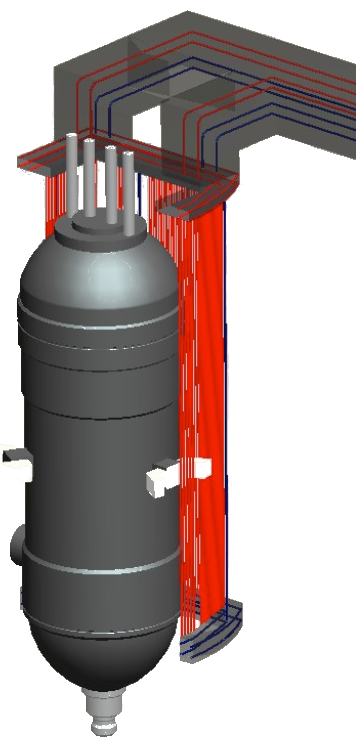
\includegraphics[scale=0.73]{RCCSMockup.png}%
\end{figure}

However, without forced cooling, the reference temperature of the entire water system will continue to rise with continued decay heat exposure.
At some point during the transient, the water leaving the riser system will reach the saturation temperature at atmospheric pressure.  
Due to the gravitational head of all the water on top of the risers, the water will not immediately boil.
Rather, as the water flows to the top of the system, it will instantly boil as it passes into a region where the local pressure falls below the saturation pressure; a process called \textit{flashing}.
This sudden discontinuous jump in substance properties results in flow oscillations because the steam produced from the flash is approximately 1,000 times less dense than the liquid state on the cold side of the system.

\Cref{Figure:RCCSFullScaleMassFlowRate} shows a numerical simulation of the full-scale system.
Before flashing, the mass flow rate is non-oscillatory and increasing due to persistent heating with no cooling.
At the onset of flashing, the flow rate rapidly oscillates and evolves in a complicated manner.
At some point in the evolution, the system's flow rate stabilizes and evolves just as the single phase system.
The period, amplitude, and overall time evolution of these oscillations is subject to numerous factors and various linear and nonlinear effects.
The oscillations are commonly referred to as density wave instabilities since they are driven by the density of the system \cite{achard_analysis_1985}.
These incessant perturbations could potentially lead to large, erratic flow excursions that could pose a safety risk via extreme mechanical or thermal damage.

\begin{figure}%
    \centering
    \caption[RCCS mass flow rate under blackout conditions]{RCCS mass flow rate versus time under blackout conditions.}%
    \label{Figure:RCCSFullScaleMassFlowRate}%
    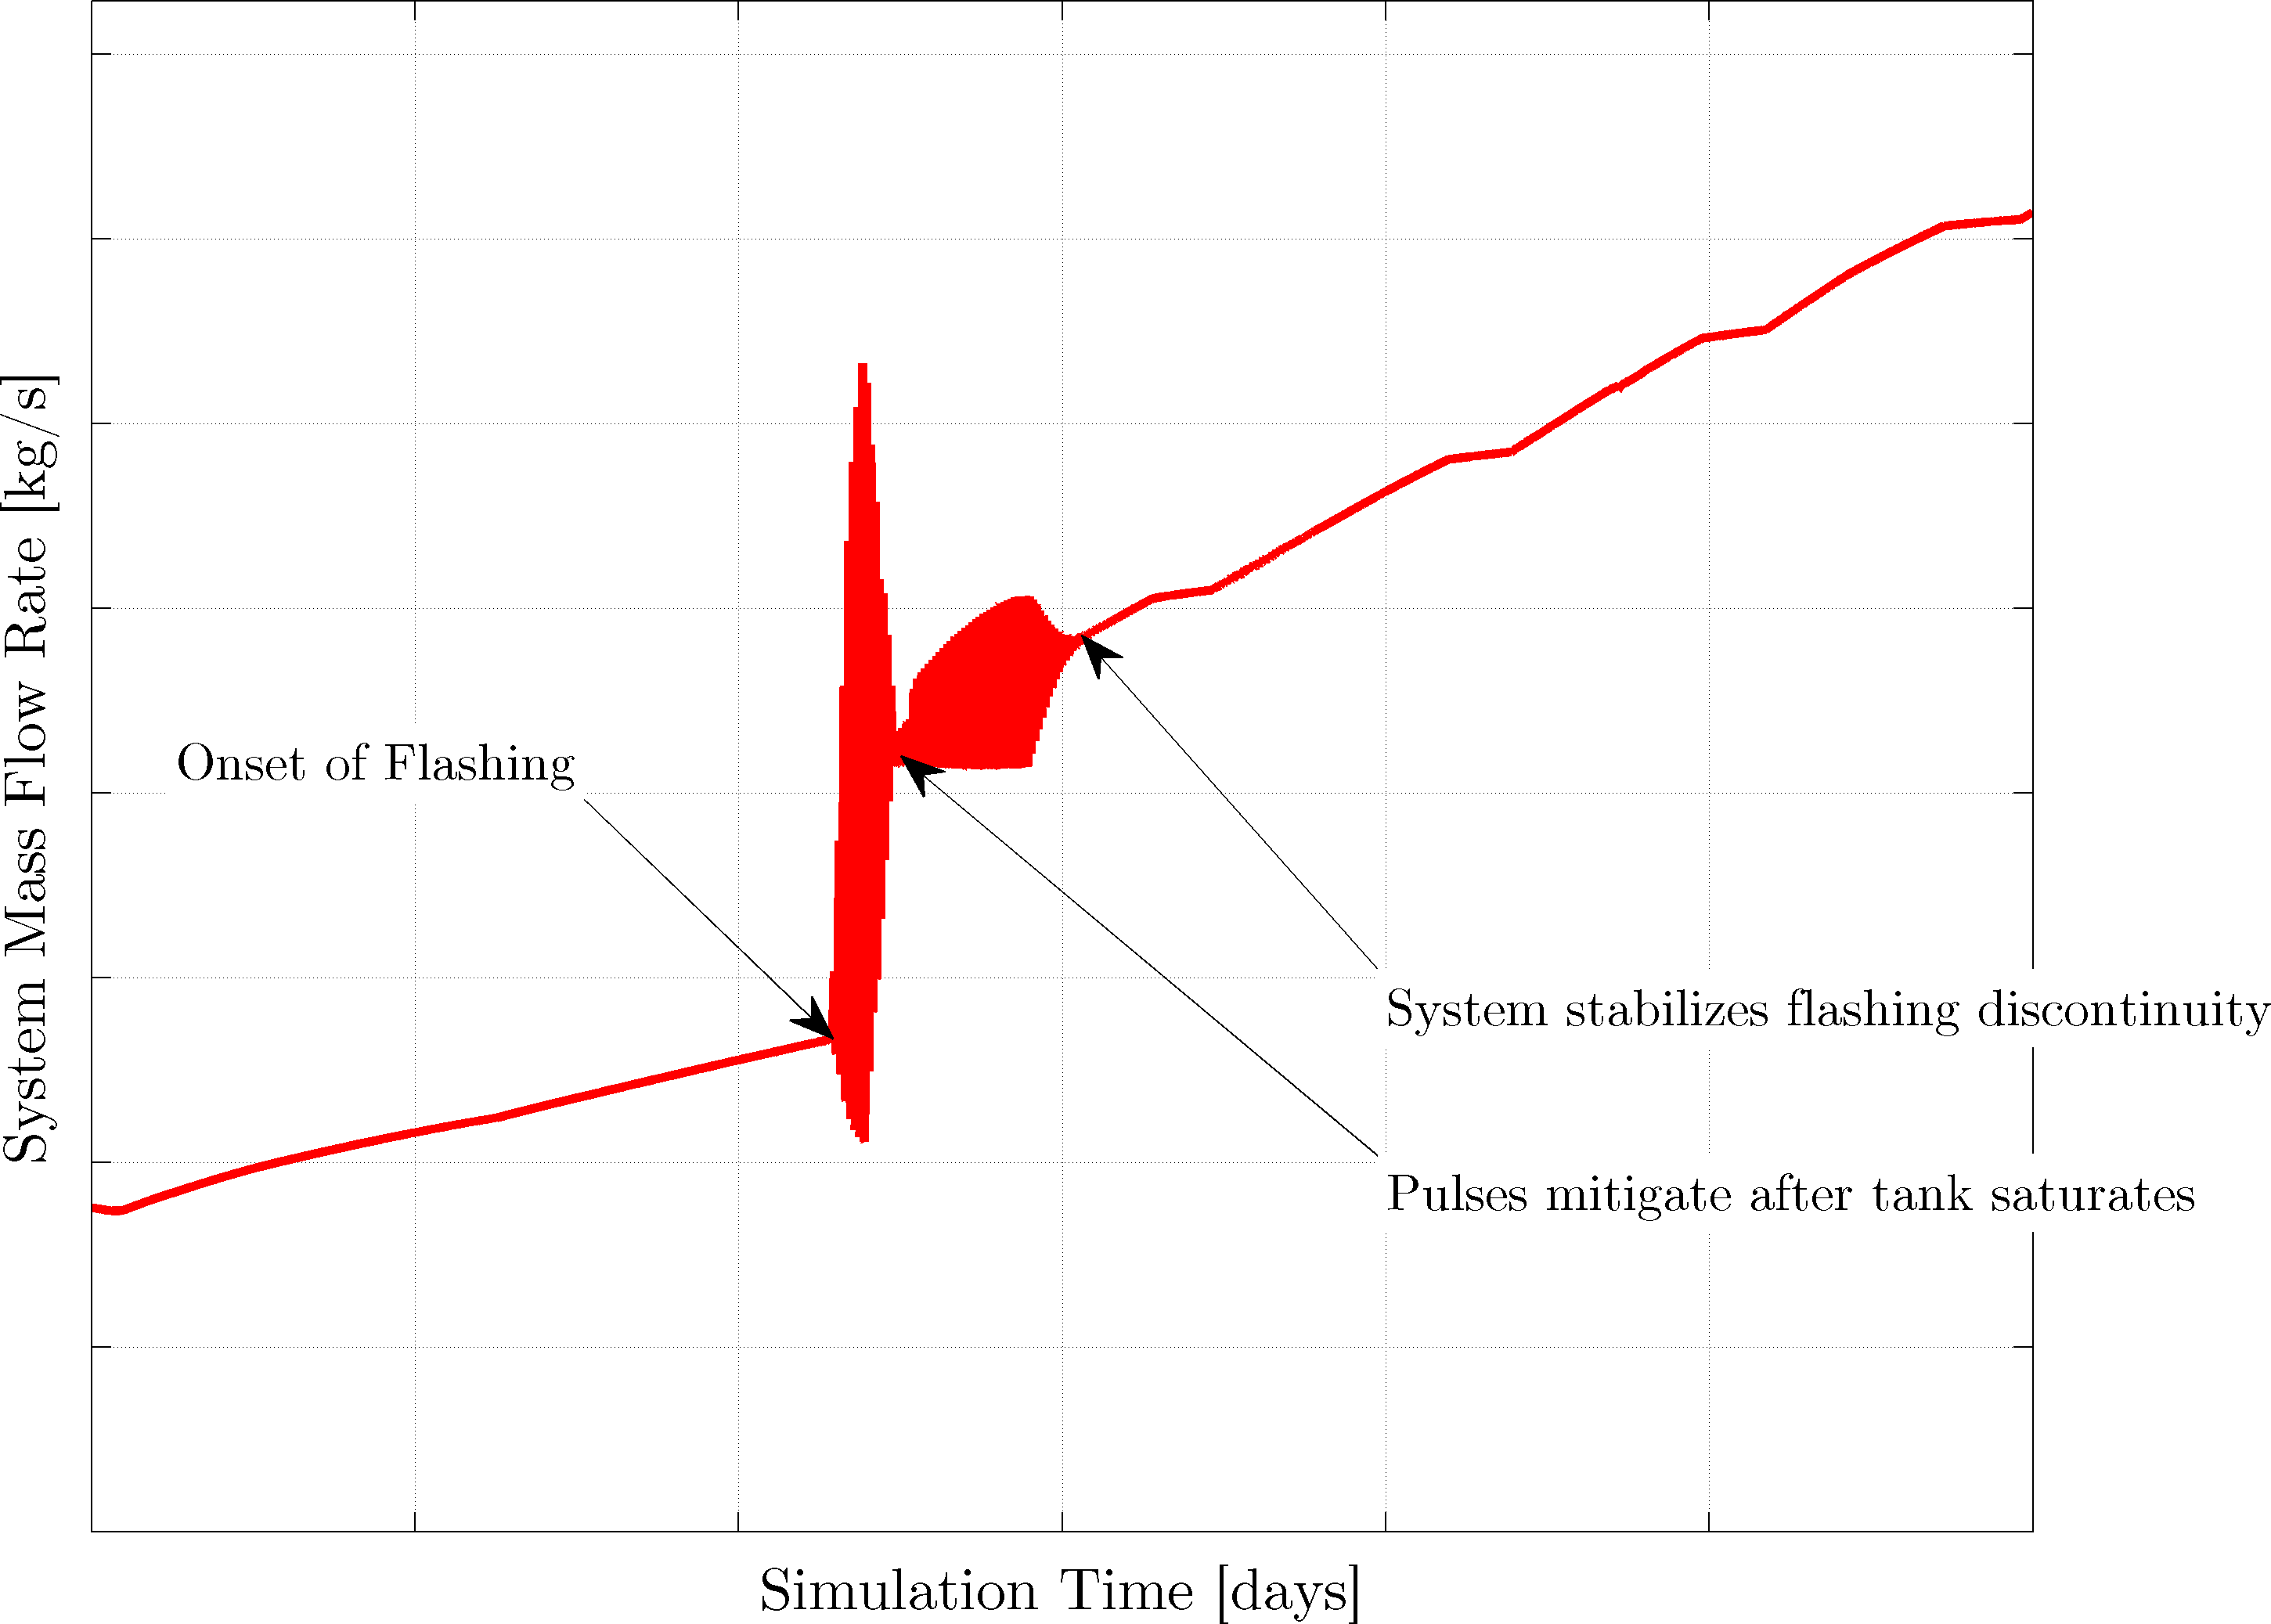
\includegraphics[width=0.9\textwidth]{PowerProfiles_MassFlowRateAnnotationsThesis.png}%
\end{figure}

\subsection{\TheUniversity\ RCCS Experiment}
Since the \Acronym{RCCS} discussed above exists purely on paper, an experiment was built at the \TheUniversity\ to directly observe and measure the behavior of an \Acronym{RCCS}-like system.
The experiment, presented in-brief by \cref{Figure:RCCSExperimentOverview}, is a scaled version of the full-scale \Acronym{RCCS} in terms of both dimension and number of risers.
While the full-scale system spans tens of meters with hundred of tubes, the experiment was scaled to a total height of approximately seven meters with three riser tubes.
Heaters mounted opposite the riser tubes provide the power to drive the natural circulation of the system.

\begin{figure}%
    \centering
    \caption[RCCS Experiment Full System diagram]{An overview of the whole RCCS experiment with important sections annotated.}%
    \label{Figure:RCCSExperimentOverview}%
    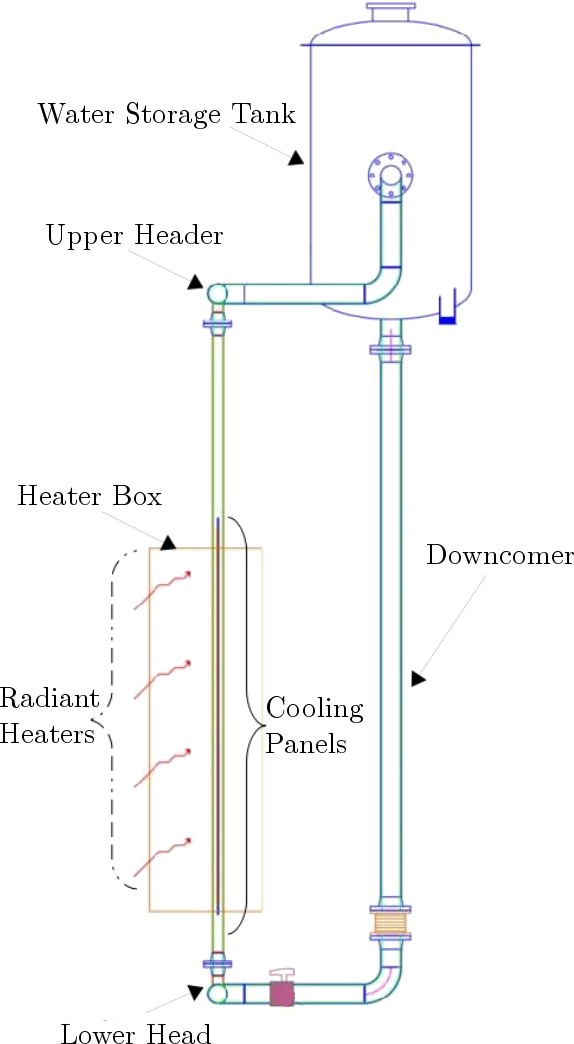
\includegraphics[height=0.50\textheight]{RCCSExperimentOverview.png}
    \vspace*{4em}
%\end{figure}%
%\begin{figure}%
    \centering
    \caption[RCCS Experiment Three Riser diagram]{An overview of the RCCS experiment's three riser/radiant heater setup.}%
    \label{Figure:RCCSExperimentHeatBox}%
    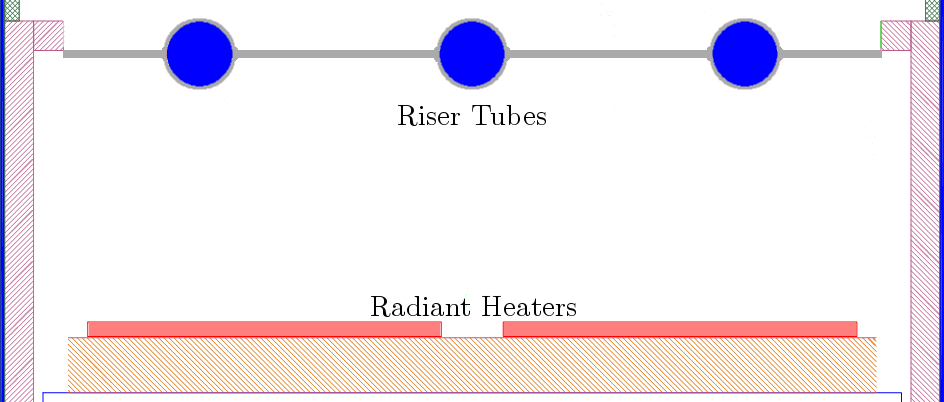
\includegraphics[width=0.80\textwidth]{RCCSExperimentHeatBox.png}%
\end{figure}

Due to the smaller scale and detailed design, a more precise numerical model could be made and benchmarked against data.
The full convection/radiation enclosure for the heater box was used to simulate station blackout conditions as in the full-scale with a scaled heat flux.
The mass flow rates from each of the risers for this accident simulation are shown in \cref{Figure:ExperimentMassFlowRateVsTime}.
The highly oscillatory nature of the flow rate after flashing begins is not only present but metastasized in this experiment.
Additionally, reverse flows in two of the risers is present (though the total system mass flow rate is always positive).
This local reversal of flow is more than likely systemic since short piping at the top allows a two-phase condition to exist at the top of the red riser.
While not expected in the full-scale system, this flow reversal is an interesting feature of the experiment's design and should be investigated.

\begin{figure}%
    \centering
    \begin{subfigure}[t]{\textwidth}
        \centering  
        \caption[ Mass flow rate versus time for the three riser tubes]{   
            Mass flow rate versus time for the three riser tubes of the RCCS experiment with station blackout accident conditions. 
            The colors of the plot lines correspond to the riser colors in \cref{Figure:RCCSExperimentRiserPlotAid}.}%
        \label{Figure:ExperimentMassFlowRateVsTime}%
        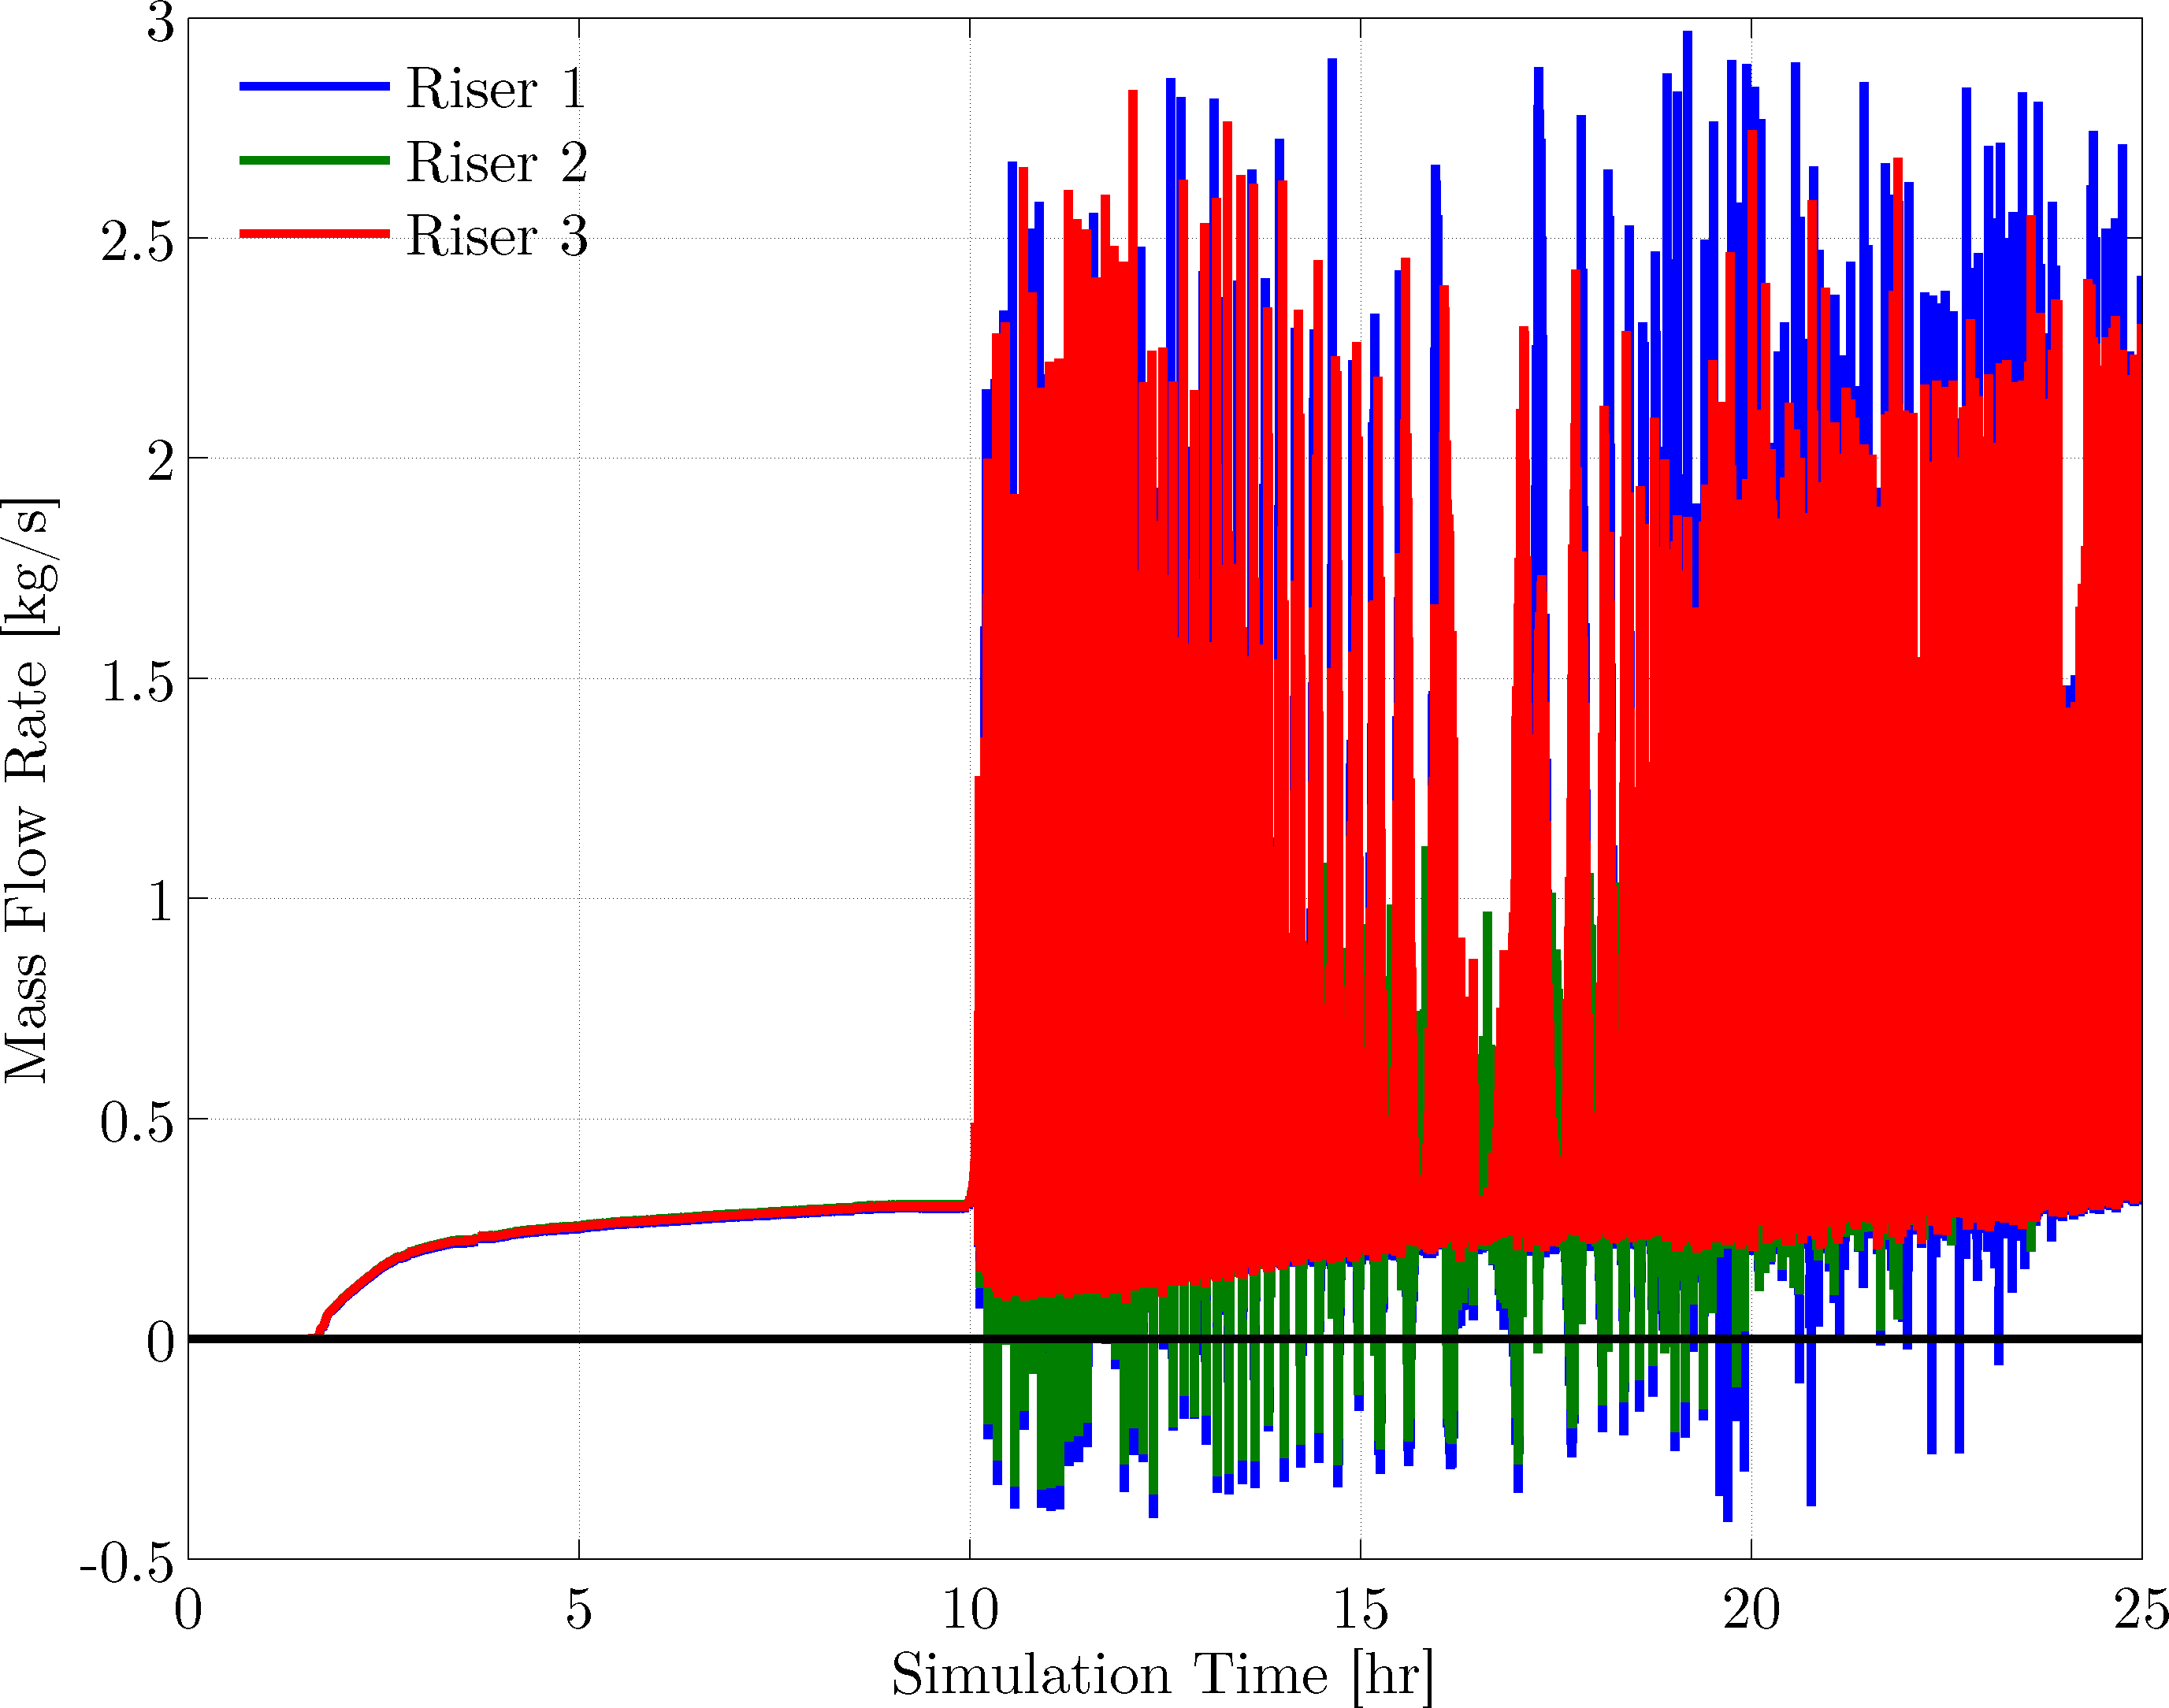
\includegraphics[width=0.75\textwidth]{ExperimentMassFlowRateVsTime.png}
    \end{subfigure}
    \vskip3em
    \begin{subfigure}[t]{\textwidth}
        \centering
        \caption[Basic layout of the RCCS experiment]{Basic layout of the RCCS experiment's numerical model.
                 The blue and red outlines denote the cooling and heating zones, respectively.}%
        \label{Figure:RCCSExperimentRiserPlotAid}%
        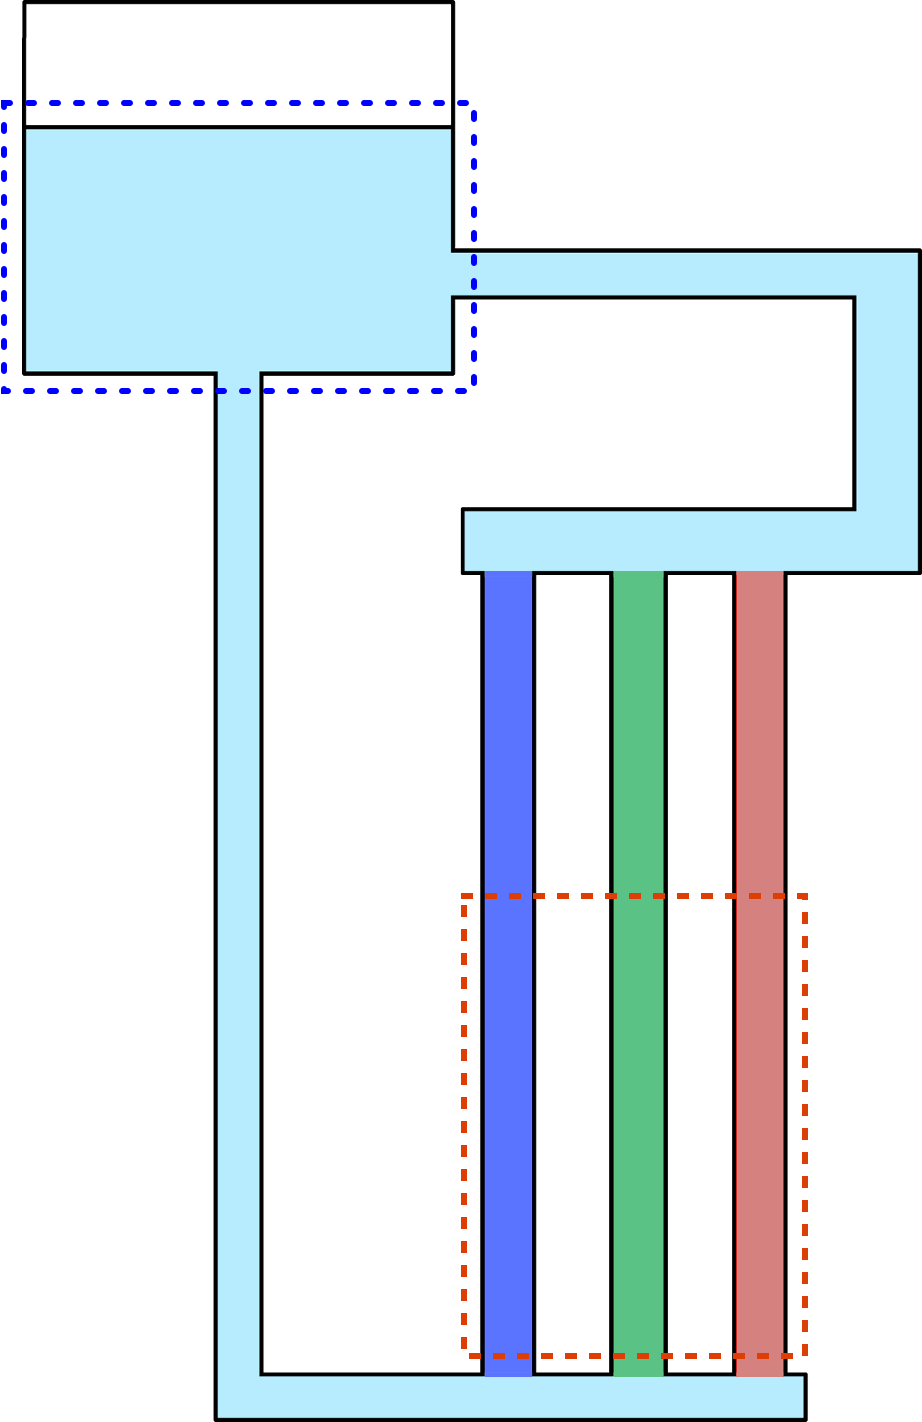
\includegraphics[height=0.35\textheight]{RCCSExperimentRiserPlotAid.png}%
    \end{subfigure}
\end{figure}

\newpage
\section{Literature}
Two-phase flow instabilities have been extensively studied across numerous industrial applications, including thermosiphons and power cycle loops; therefore, the literature of two-phase flow instabilities is extensive.
It should be noted that single phase instabilities do exist and are researched \cite{satoh_instability_1998}, but an in-depth overview of those mechanisms will not be given.
An overview of two-phase instabilities, classifications, and definitions is given below.
Then, specific discussion of efforts and techniques of analysis is discussed.

\subsection{Two-Phase Flow Instabilities}
There are a variety of ways to classify two-phase flow instabilities depending on geometry, spatial/temporal dependence, multiphase models, etc.
Difficulties also arise when real world applications see a confluence of all of these parameters.
Both Boure \etal\ and Kakac \etal\ provide extensive discussions of general two-phase flow instability characterization \cite{boure_review_1973,kakac_review_2008}, and their similar systems for describing two-phase will be used throughout this section.
\Cref{Table:StaticInstabilities,Table:DynamicInstabilities} present a summary of general two-phase instabilities presented by the above authors; however, not all of them will be discussed in detail.
Presad \etal \cite{durgaprasad_review_2007} and Nayak \etal \cite{nayak_flow_2008}, while overlapping somewhat with the generic descriptions of instabilities, present and classify certain instabilities as natural circulation specific that should be described.
Most of the following discussion concerns a flowing fluid undergoing phase transition in a channel which may require some familiarity with two-phase flow regimes; explanation of these regimes is left to the literature (\eg \cite{thome_chapter_2004,tong_boiling_1997,ghiaasiaan_twophase_2007}).


Key terms are now given specific definitions for clarity.
If a system at steady-state is perturbed and eventually returns to its initial equilibrium, the system is described as \textit{stable}.
If a system at steady-state is perturbed into a neighborhood where no equilibrium exists near the initial state, the system possesses a \textit{static instability}.
A system has \textit{dynamic instabilities} if there are inherently transient feedback mechanisms that may lead to a steady-state, though there is no guarantee of uniqueness.
An instability that arises from another is referred to as a \textit{secondary phenomenon} (the instigator being the primary).
\textit{Fundamental instabilities} are those which exhibit one primary mechanism.
\textit{Compound instabilities} is one that incorporates two or more mechanisms that confound separate analysis.
\cref{Figure:StabilityBAH} defines through illustration several other forms of stability through a ball-and-hill physical analogy.

One aspect of the stability the above definitions do not discuss is the magnitude of the system perturbations.
The strength of the perturbation is important since it determines how much energy is imparted into the system and, therefore, how far the system will travel from its initial state.
The importance can be seen in \cref{Figure:StabilityBAH:LUNS,Figure:StabilityBAH:LSNU} where both systems exhibit different behavior depending how hard the system is ``hit''.
\Cref{Figure:StabilityBAH:LUNS} shows a linear instability while actually being nonlinearly stable with multiple equilibria.
\Cref{Figure:StabilityBAH:LSNU} exhibits linear stability while being nonlinearly stable
These concepts are important to consider when looking at linear stability because the behavior beyond the system's linear boundary is technically \textit{terra incognita}.
Actually performing a nonlinear analysis, if possible, is the only surefire tool for assessing stability.

\begin{figure}%
    \centering%
    \caption[Ball-and-hill analogy of equilibrium descriptions]{
                Ball-and-hill analogy of equilibrium descriptions.  
                The ball represents some state at a given time and place, and 
                the shapes supporting the ball dictate how the state moves when subjected to a perturbation.
                Troughs are considered stable while crests/runoffs are unstable.}%
    \label{Figure:StabilityBAH}%
    %
    %
    \begin{subfigure}[t]{0.48\textwidth}
        \centering
        \caption{Neutral equilibrium (infinitely many steady-states)}
        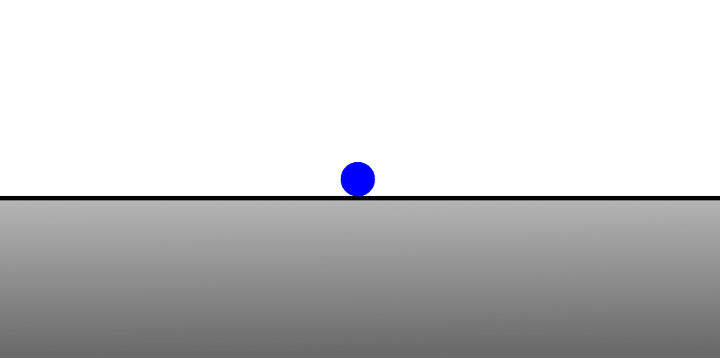
\includegraphics[height=1.3in]{NeutralEquilibirum.png}
        \label{Figure:StabilityBAH:Neutral}
    \end{subfigure}
    \hfill
    \begin{subfigure}[t]{0.48\textwidth}
        \centering
        \caption{No equilibrium (no steady-state)}
        \label{Figure:StabilityBAH:None}
        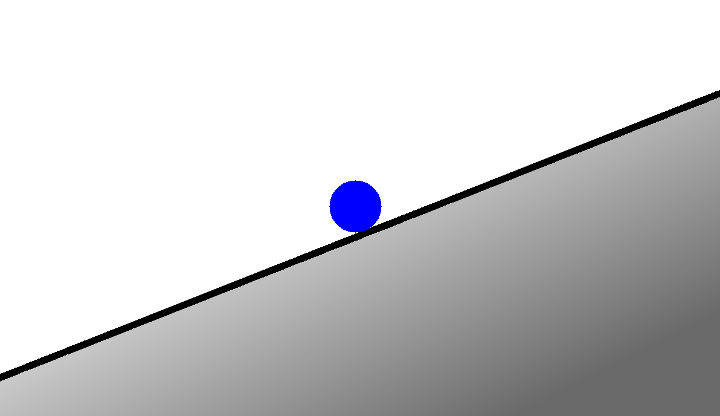
\includegraphics[height=1.3in]{NoEquilibirum.png}
    \end{subfigure}
    %
    \vskip4em
    %
    \begin{subfigure}[t]{0.48\textwidth}
        \centering
        \caption{Stable equilibrium}
        \label{Figure:StabilityBAH:Stable}
        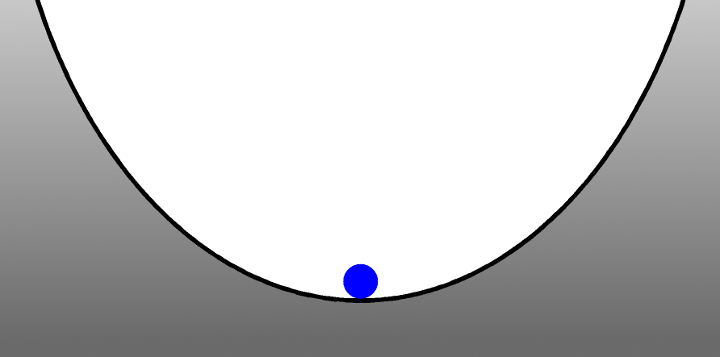
\includegraphics[height=1.3in]{Stable.png}
    \end{subfigure}
    \hfill
    \begin{subfigure}[t]{0.48\textwidth}
        \centering
        \caption{Unstable equilibrium}
        \label{Figure:StabilityBAH:Unstable}
        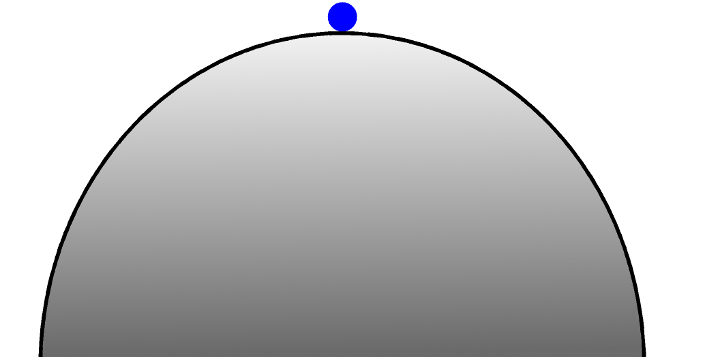
\includegraphics[height=1.3in]{Unstable.png}
    \end{subfigure}
    %
    \vskip4em
    %
    \begin{subfigure}[t]{0.48\textwidth}
        \centering
        \caption{Linearly unstable, nonlinearly stable equilibrium}
        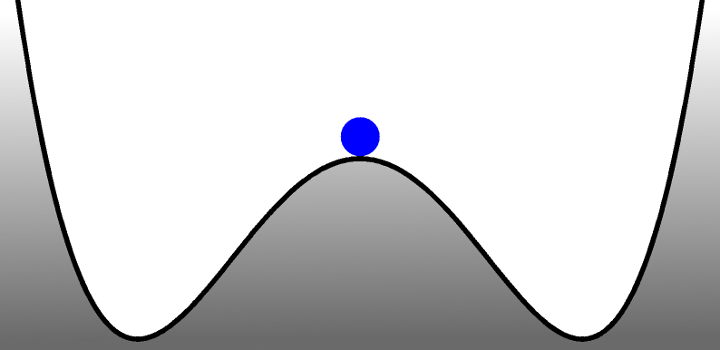
\includegraphics[height=1.3in]{LinearlyUnstableNonlinearlyStable.png}
        \label{Figure:StabilityBAH:LUNS}
    \end{subfigure}
    \hfill
    \begin{subfigure}[t]{0.48\textwidth}
        \centering
        \caption{Linearly stable, nonlinearly unstable equilibrium}
        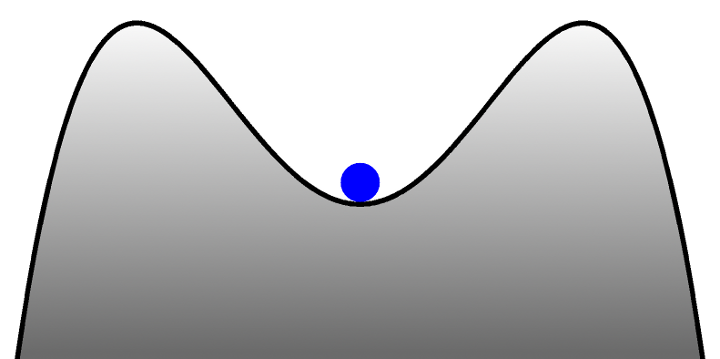
\includegraphics[height=1.3in]{LinearlyStableNonlinearlyUnstable.png}
        \label{Figure:StabilityBAH:LSNU}
    \end{subfigure}
    %
    %
\end{figure}


\subsubsection{Static Instabilities}
Static instabilities are characterized by either a pure steady-state analysis or an analysis that foresees dynamic feedback from the steady-state system.
The analysis tools used to derive stability boundaries for these instabilities will be discussed in \cref{Section:StabilityTheory}.

A flow excursion, also known as a Ledinegg instability, is the sudden drop in a steady flow rate to a lower, steady value.
This jump occurs when the pressure losses in a system decrease with increasing flow rate.
For a liquid undergoing phase change in a channel, there is a complex, internal relationship between the buoyancy, friction, and acceleration momentum terms that must be taken into account for steady flow.
If the flow is forced by external sources and the internal forces of the flow are not properly taken into account, then the pressure drop could rise with increasing flow; this is especially true for slightly sub-cooled flows entering a heated region where a sudden change in void fraction can have a large impact on the flow behavior with the system.

Fundamental relaxation instabilities occur when two or more flow regimes have state equilibriums close to each other.
For example, a bubbly flow that experiences a small change in flow rate could transition to the annular regime.
Then, the flow rate will experience an increase since annular flow has a relatively low pressure drop, and the flow regime transitions back to the bubbly regime.
Given the right situation, this cycle could continue ad infinitum.
The flow regime transitions act as a relaxation mechanism (in the dynamical system sense) that causes persistent, periodic behavior.

Chugging is an instability associated with the jetting of large vapor structures from a flow channel into larger space.
This instability typically occurs with low velocities and moderate void fractions \cite{tong_boiling_1997}.
A flowing liquid receiving heat may development large vapor bubbles in a coolant channel; this increases the flow rate due to the vapor-to-liquid ratio.
After the bubbles have been expelled, and possibly quenched, at the channel exit, the flow rate will return to the pre-slug rate.
As with the relaxation instability, this mechanism also has a periodic nature \cite{aritomi_geysering_1993}.



\subsubsection{Dynamic Instabilities}
Dynamic instabilities, unlike static, are inherently transient and primarily involve the transmission of information via waves.
As is discussed further in \cref{Chapter:Theory}, \THs systems typically possess a material (or density) wave and an acoustic (or pressure) wave.
For a non-ideal fluid, the acoustic wave's speed is primarily a function of the system's density and temperature while the material wave travels near the physical speed of the system.

Acoustic instabilities are typically of high frequency ($10$Hz--$10$kHz) and have been observed in various boiling regimes.
The acoustic waves were found to cause large pressure drop oscillations relative to steady-state values.
Even in situations where the lower frequency density waves were present, there was a clear superposition of high frequency acoustic waves with the material waves.
At high pressure-and-temperature water experiments, the acoustic waves reached frequencies that were clearly audible (so-called whistler modes).

Material wave instabilities are the most common in two-phase flow and are a highly physical phenomenon that occur from a complex coupling of \THs equations, constitutive relations, and geometry.
These waves have also been described as ``flow-void feedback instabilities'' for boiling systems \cite{neal_mechanisms_1967} and ``time-delay oscillations'' due to the relatively slow transmission of information at material speed \cite{boure_oscillatory_1966}.
Since the oscillation has its roots in the differing densities of a fluid's liquid and gas phases, vertical channel height (where the system pressure changes greatly with position), inlet conditions (thermodynamic and kinematic), and total heat transfer between the fluid and the surroundings are extremely important in the control and appearance of these flow oscillations.
It has been found that by increasing the system pressure these oscillations can be mitigated or eliminated since the density ratio of the competing phases approach one another as the pressure increases.

These material oscillations can lead to oscillations in the boiling heat transfer processes at the wall and results in a compound thermal instability.
The emphasis here is put on the highly variable nature of the two-phase heat transfer coefficient at the wall and how the information being propagated from the wall interacts with material wave oscillations.
The effects of this interaction can be as bad as an oscillating dry point in the channel with large temperature oscillations.



\subsubsection{Natural Circulation Instabilities}
There are two natural circulation instabilities of primary interest: flashing and compound natural circulation.
As mentioned in \cref{Section:RCCS}, flashing occurs when a high temperature liquid flows into a region of lower pressure such that it enters a saturated or superheated state and immediately bursts into a two-phase mixture.
This mechanism is a primary cause of material wave instabilities in natural circulation loops at low pressures or long vertical channels.
This type of instability is currently under examination for one and two protypic fuel channels \cite{marcel_experimental_2009,marcel_experimental_2010}.

The final instability is the compound natural circulation instability.
This instability is the confluence of vertical channel heating, material wave oscillations (possibly due to flashing), chugging phenomenon, and flow regime transitions.
Since the system's flow rate is not subject to any mechanical head contributions, all of these instabilities can occur concurrently and must be carefully analyzed to discern which of the mechanisms are present and which is dominate.
These instabilities are extremely important for all types of nuclear reactors and are under continuously under investigation \cite{dauria_characterization_1990,aritomi_fundamental_1992,yun_twophase_2005}.

\begin{table}
    \centering
    \caption[Summary of static flow instabilities]{Summary of static flow instabilities due to \cite{boure_review_1973}}
    \label{Table:StaticInstabilities}
    \rowcolors{2}{}{Gray}
    \setstretch{1.05}
    \renewcommand{\arraystretch}{1.4}
    {\small
    \hyphenation{Transition}
    \hyphenation{Relaxation}
    \begin{tabular}{>{\centering}p{1.15in} >{\centering}p{1.1in}  >{\raggedright}p{1.4in}  >{\raggedright\arraybackslash}p{1.5in} }
        \toprule
        \multicolumn{1}{c}{\textbf{Name}}      & \multicolumn{1}{c}{\textbf{Class}} & 
        \multicolumn{1}{c}{\textbf{Mechanism}} & \multicolumn{1}{c}{\textbf{Characteristics}}\\\midrule
        % --------------------------------------------------------------------------------- 
        Flow excursion                     & Fundamental            & 
                \LedineggCriterion & Sudden, large flow change to a new, stable state \\
        % ---------------------------------------------------------------------------------
        Boiling crisis                     & Fundamental            & 
                Ineffective cooling & Wall temperature excursion and flow oscillation \\
        % ---------------------------------------------------------------------------------
        Flow Regime  Transition             & Fundamental Relaxation & 
                Varying $\Delta{P}$ between regimes            & Cyclic flow pattern transitions and flow rate variations \\
        % ---------------------------------------------------------------------------------
        Bumping, geysering, or    chugging & Compound    Relaxation & 
                Periodic adjustment of metastable conditions & Periodic superheat and violent evaporation \\
    \bottomrule
    \end{tabular}
    }
\end{table}
\begin{table}
    \centering
    \caption[Summary of dynamic flow instabilities]{Summary of dynamic flow instabilities due to \cite{boure_review_1973}}
    \label{Table:DynamicInstabilities}
    \rowcolors{2}{}{Gray}
    \setstretch{1.05}
    \renewcommand{\arraystretch}{1.4}
    {\small
    \hyphenation{Compount}
    \hyphenation{Relaxation}
    \begin{tabular}{>{\centering}p{1.1in} >{\centering}p{1.1in} >{\raggedright}p{1.55in} >{\raggedright\arraybackslash}p{1.55in} }
        \toprule
        \multicolumn{1}{c}{\textbf{Name}}      & \multicolumn{1}{c}{\textbf{Class}} & 
        \multicolumn{1}{c}{\textbf{Mechanism}} & \multicolumn{1}{c}{\textbf{Characteristics}}\\\midrule
        % --------------------------------------------------------------------------------- 
        Acoustic  Oscillations  & Fundamental & Resonance of pressure waves & 
                High frequency oscillations near the acoustic speeds\\
        % ---------------------------------------------------------------------------------
        Density Wave  Oscillations  & Fundamental & Coupled mass, momentum, and energy feedback & 
                Low frequency oscillations near the material speed\\
        % ---------------------------------------------------------------------------------
        Thermal  Oscillations  & Compound & Variable heat transfer coefficient interacting with flow & 
                Occurs during film boiling \\
        % ---------------------------------------------------------------------------------
        BWR  Instability &  Compound & Hydraulic-neutronic coupling & 
                Strong only for a small fuel time constant and low pressure\\
        % ---------------------------------------------------------------------------------
        Parallel  Channel  Instability & Compound & Interaction among parallel channels & 
                Various modes of flow redistribution\\
        % ---------------------------------------------------------------------------------
        Pressure drop  Oscillations & Secondary Compound& 
                Flow excursions initiate interactions between channels and compressible volumes & 
                        Very low frequency, periodic process\\
    \bottomrule
    \end{tabular}
    }
\end{table}
\begin{table}
    \centering
    \caption[Effects of parametric variation on instability]
            {Effects of parametric variation on instability for a flow entering a vertical channel sub-cooled or saturated 
             due to \cite{durgaprasad_review_2007}}
    \label{Table:ParametericEffects}
    \rowcolors{2}{}{Gray}
    \setstretch{1.05}
    \renewcommand{\arraystretch}{1.5}
    {\small
    \hyphenation{Transition}
    \hyphenation{Relaxation}
    \begin{tabular}{>{\centering}p{1.6in} >{\raggedright}p{1.3in} >{\raggedright\arraybackslash}p{2.8in}}
        \toprule
        \multicolumn{1}{c}{\textbf{Parameter Increased}}  & \multicolumn{1}{c}{\textbf{Effect}} & 
        \multicolumn{1}{c}{\textbf{Reason}}\\\midrule
        % --------------------------------------------------------------------------------- 
        System pressure & Stability increases & Phase density difference lessens thus reducing the gravitational head gain. \\
        % ---------------------------------------------------------------------------------
        Mass flow rate  & Stability increases & Critical power for oscillation generation increases and avoids chugging.\\
        % ---------------------------------------------------------------------------------
        Inlet sub-cooling& Destabilizes at small sub-coolings but stabilizes otherwise &
                For small sub-coolings,due to significant response delay in void formation with an increase in transit time.
                Otherwise, it reduces void fraction and increases non-boiling length.\\
        % ---------------------------------------------------------------------------------
        Inlet resistance & Stability increases & Increases the single phase friction which has a damping effect upstream.\\
        % ---------------------------------------------------------------------------------
        Exist resistance & Stability reduces   & Increases two-phase friction which amplifies instabilities upstream\\
        % ---------------------------------------------------------------------------------
        Riser height     & Stability reduces   & 
                Increases two-phase gravitational pressure drop and phase transition as static head decreases\\
    \bottomrule
    \end{tabular}
    }
\end{table}


\newpage
\subsection{Previous Analysis Efforts}
The two main types of analysis employed in stability analysis are linear and nonlinear, a superset of the former.
Every analysis begins with a defined set of the conservation/balance equations.
These equations possess all of the modeling information and assumptions in the analysis to be performed.
Three commonly used models are \cite{johnson_handbook_1998}:
\begin{itemize}
    \item{a homogeneous equilibrium model (HEM) where the distinct phases of a boiling fluid are treated as a single fluid with averaged properties;}
    \item{a separated flow model (SFM) where an additional momentum equation is added to the HEM allowing phase slip;}
    \item{a two-fluid model where the distinct phases are treated as separate partitions of a total volume, have completely separate properties, and only communicate through their shared interface.}
\end{itemize}
\Cref{Chapter:Theory} discusses the HEM and two-fluid equations, but for now, it suffices to say that these equations are nonlinear, coupled partial differentials equations that do not, in general, admit analytical solutions.

After the model has been decided, authors either linearize the equations or not and assess the system's stability through various techniques.
The specifics of the solution techniques are left to \cref{Section:StabilityTheory} since the techniques are all similar.
What makes the approaches more interesting is the models used, approximations made, and geometry considered.

Wallis and Heasley present one of the earliest efforts to analytically tackle two-phase flow oscillations \cite{wallis_oscillations_1961}.
They investigated a simple, closed natural circulation loop with pentane as the working fluid.
The analysis method looked at three sources of oscillations from a Lagrangian frame.
The first source was changes in riser buoyancy resulting from velocity perturbations and an equation for the marginal stability was derived in terms of the friction factor's derivative with respect to some steady-state velocity.
The second source was the heat input into the system with a theorized flow excursion for their loop.
Lastly, they investigated parallel channels but did not complete the analysis due to the then intractability of the solution.

Welander, though not a study of two-phase instabilities, investigates a simple, closed loop with point sources and proportional constitutive relations.\cite{welander_oscillatory_1967}.
While the treatment is similar to Wallis and Heasley's, Welander's more mathematical approach is more in-line with this work's goals.
Additionally, Welander derived an asymptotic steady-state solution and also compared the analytical neutral boundary with numerical experiments to confirm the boundary's validity.
Zvirin and Greif continued this work by examining how an arbitrary initial condition evolved toward Welander's steady state \cite{zvirin_transient_1979}.
They found that while the solution approached the analytical steady-state, the solution was without oscillation and concluded that the oscillation characteristics were strongly dependent on the shape of the initial condition.

Achard \etal investigated material wave oscillations in a horizontal boiling channel using both linear and nonlinear analysis \cite{achard_analysis_1985}.
They derived a lumped parameter integrodifferential equation.
Upon linearizing the equation and using the friction and sub-cooling numbers as degrees of freedom, they found two absolutely unstable regions, several conditionally unstable regions, and one absolutely stable region.
The conditionally unstable regions were found to depend on how actual system's state evolved in time and moved through the stability space.
They also performed a nonlinear analysis where the parameter values to maintain stability were obtained by nonlinearly solving the lumped parameter equation for a given perturbation amplitude.
The nonlinear analysis showed that stable parameter curves existed for their system but the absolutely stable region shrank with increasing perturbation amplitude.

Lee and Ishii performed a linear analysis similar to Welander, but the system was explicitly two-phase, had a quadratic frictional dependence in velocity with a constant friction factor, and had a distributed heat load \cite{sangyonglee_thermally_1990}.
Additionally, as an extension of the Zvirin and Greif's methodology, Lee and Ishii divided the loop into size different regions with average properties and solved for the stability boundary using linear analysis.

Lee and Lee performed nearly the same analysis as Lee and Ishii with the added difficulty of a variable, flow-regime dependent friction factor \cite{lee_linear_1991}.
Guanghui \etal also performed a similar analysis over a simple, closed loop that compared very well experiments \cite{guanghui_theoretical_2002}.

Knaani and Zvirin investigated the existence of multiple steady-states for a simple, closed loop undergoing boiling\cite{knaani_bifurcation_1993}.
The analysis was done with HEM and incorporated a guess and check procedure for finding a solution to the nonlinear problem.
They ultimately found multiple steady-states for the closed system due to the non-monotonic nature of the buoyancy term during phase change.
Nayak \etal also performed analysis on a simple, closed loop but used a four equation model (two for mass and mixture equations for energy and momentum) and several different two-phase friction multipliers \cite{nayak_study_2007}.

Lee and Pan undertook an \Acronym{HEM} for a two-phase natural circulation system with two parallel, heated channels \cite{lee_nonlinear_2005}.
This treatment is the first work in this review to explicitly analyze a non-simple closed loop.
Through a number of piece-wise integrations along the loop, the authors arrived at a set of ordinary differential equations that satisfied the zero pressure gradient requirement of the closed loop.
Using the channel inlet sub-cooling as a parametric and a blackbox solver, the authors compared the steady-state channel flow rates with experimental data.
The authors then found a stability curve for even heating of the channels that possessed two unstable regions and one stable region.
The author concluded with a parametric study of how the stability region shifted with the addition of an orifice plate.










\section{Research Purpose}\label{Section:Purpose}

The purpose of this research is to theoretically investigate the linear stability of a closed loop, natural circulation system undergoing phase-change with water as a working fluid.
The goal is to ultimately apply stability theory to three parallel channels in a closed circuit with mass loss, which form a novel combination for the literature.
As the system boils, the inventory is draining and a question that has not been completely answered is how does this affect the stability and overall evolution of the system.
In addition to the geometrical considerations, this work also explores a novel discretization scheme to the standard set of thermohydraulic equations that aims to more accurately represent branching flows than standard channel flow models.
Also, this work applies a full non-linear solver to the set of discretized equations with no operator splitting over a time-step.
Lastly, the linear stability of the system over a transient is determined through a detailed volume integration of the governing equations and an eigenvalue calculation.

The outline of the topics to be discussed in this work is:
\begin{enumerate}[topsep=0pt,parsep=0pt,itemsep=2pt]
    \item{conservation laws and pertinent thermohydraulic equations to solve;}
    \item{the discretization scheme and approximations applied to the equations;}
    \item{stability theory as applied to the set of nonlinear equations;}
    \item{the nonlinear solver used;}
    \item{results of transient simulations and associated stability calculations;}
    \item{conclusions from the presented results and future work.}
\end{enumerate}
Each section builds upon the last and works to fulfill the delineated goals above.



\bibliography{../Sources}
\bibliographystyle{unsrt}

 
 \fi

\end{document}




